\chapter{Fundamentação Teórica}\label{cap:fundamentacao}

Reúnem-se neste capítulo os conceitos necessários para entender o que este trabalho realizou e
como ele se insere no que já foi feito na área. A \autoref{sec:revisao} percorre a
literatura sobre padrões de escoamento bifásico e sobre o uso da transformada
\textit{Wavelet} em sinais de escoamento. A \autoref{sec:bases} apresenta os fundamentos
teóricos que sustentam a metodologia: o comportamento do escoamento bifásico em
microcanais e a formulação matemática das transformadas \textit{Wavelet}, incluindo a
formulação alternativa de coerência aplicada neste trabalho.

% =========================================================
\section{Revisão Bibliográfica}\label{sec:revisao}
% =========================================================

Esta seção percorre os principais trabalhos relacionados ao tema deste trabalho, com o
objetivo de situar a proposta dentro do contexto da literatura e identificar a lacuna
que justifica o trabalho.

% ---------------------------------------------------------
\subsection{Padrões de escoamento bifásico em microcanais}\label{sec:rev-padroes}
% ---------------------------------------------------------

Quando um fluido evapora dentro de um tubo de pequeno diâmetro, as duas fases não formam
uma mistura uniforme. Líquido e vapor se organizam em configurações geométricas distintas,
os chamados padrões de escoamento, que mudam conforme a quantidade de vapor presente e a
velocidade do fluido. À medida que o diâmetro diminui, os efeitos de confinamento e a
importância relativa da tensão superficial aumentam, alterando os padrões e as
condições de transição \cite{cheng2023}.

\citeonline{deoliveira2019} investigaram as séries temporais do sensor óptico durante a
ebulição convectiva de hidrocarbonetos (R-600a, R-290 e R-1270) em tubo horizontal
de 1\,mm, a 17\textdegree{}C de temperatura de saturação, com fluxo mássico entre 240 e
480\,kg/(m\textsuperscript{2}s) e fluxo de calor entre 5 e 60\,kW/m\textsuperscript{2}.
Cinco padrões foram identificados e suas frequências características analisadas por
transformada de Fourier e por métricas de não-linearidade, incluindo expoentes de Lyapunov
e retratos de fase. Os resultados indicaram comportamento caótico em todos os padrões e
frequências características distintas associadas à morfologia da interface líquido-vapor.

\citeonline{deoliveira2021} realizaram um estudo experimental mais amplo no mesmo arranjo,
com isobutano (R600a), identificando seis padrões de escoamento. Além do
sensor óptico (OS), analisaram-se as flutuações do transdutor de pressão diferencial
(PD), já presente no arranjo de 2019. A aquisição simultânea permitiu comparar
respostas complementares: a análise por transformada \textit{Wavelet} contínua (CWT)
identificou frequências características
em diversas condições, mas não uma assinatura exclusiva de cada padrão em ambos
os sensores. Essas respostas são descritas na \autoref{sec:padroes}. Os parâmetros
experimentais completos estão listados no \autoref{qua:params-exp}.
Esse estudo fornece a descrição do arranjo experimental considerado neste trabalho.
A análise CWT utilizou um algoritmo adaptado de \citeonline{torrence1998},
conforme explicitado no artigo de \citeonline{deoliveira2021}.

\citeonline{schmid2022} mapearam padrões de escoamento adiabático de
CO\textsubscript{2} em tubo vertical de 8\,mm, nas direções ascendente e
descendente. O estudo mostrou a influência do título de vapor $x$, do fluxo mássico $G$
e da direção do escoamento sobre os padrões observados. Esses resultados
ressaltam a necessidade de considerar as condições de cada arranjo ao comparar
mapas de padrões com os de ebulição horizontal de R600a deste trabalho.

% ---------------------------------------------------------
\subsection{Análise por transformada \textit{Wavelet} em escoamentos bifásicos}\label{sec:rev-wavelet}
% ---------------------------------------------------------

\citeonline{torrence1998} apresentaram um guia prático de análise \textit{Wavelet} contínua
para séries temporais, com ênfase no espectro de potência \textit{Wavelet} (WPS) e em
métodos para avaliar a significância estatística dos resultados. O artigo também introduz
o espectro cruzado (WCS) e discute as limitações do estimador clássico de coerência
\textit{Wavelet} (WCO). A localização em tempo e frequência complementa o espectro
de Fourier global quando o conteúdo espectral varia ao longo do registro.

Um antecedente direto da abordagem adotada neste trabalho foi desenvolvido por
\citeonline{nguyen2010}, que aplicaram a CWT a sinais de fração de vazio em escoamento
bifásico vertical ar-água em tubo de 80\,mm (laboratório KAERI, Coreia). Os autores
combinaram a energia efetiva da CWT, a razão entre o comprimento efetivo estimado
da estrutura gasosa e o diâmetro do tubo, usando a escala efetiva e a velocidade de propagação,
e a fração de vazio média.
Com esses critérios, distinguiram quatro sub-regimes: \textit{discrete bubbly},
\textit{clustered/cap bubbly}, \textit{slug} e \textit{churn}. O resultado
mostra a utilidade de combinar descritores locais da CWT com informações
físicas do escoamento.

\citeonline{morshed2020} aplicaram decomposição por pacotes \textit{Wavelet}
com base db4 a sinais de pressão em escoamentos ar-água e ar-solução de
goma xantana. A entropia de norma evidenciou características dos regimes de
bolhas, de transição entre bolhas e bolhas alongadas e de \textit{slug}, com
limitações de resolução e resposta em frequência do sensor.
\citeonline{tan2015} combinaram sensores de
condutância e capacitância com análise por transformada \textit{Wavelet} contínua (CWT) e
demonstraram que os coeficientes de energia \textit{Wavelet} local (LWE) constituem
descritores das estruturas e transições do escoamento óleo-água, embora os autores
ressaltem que a distribuição característica obtida é específica para o arranjo e fluidos
utilizados (tubo de 50\,mm, óleo branco e água).

\citeonline{sun2012} aplicaram decomposição \textit{Wavelet} e entropia de norma
sobre flutuações de pressão diferencial em escoamento bifásico ar-água horizontal
(tubo de 50\,mm). Os mapas combinaram a entropia de norma média com a vazão mássica
total ou com a fração volumétrica de gás calculada a partir das vazões das fases.
Obtiveram taxas globais de identificação de 98{,}0\% e 95{,}9\%, respectivamente,
para quatro padrões. Nessa avaliação,
pontos sobre as fronteiras receberam meio erro. Esses antecedentes motivam a
investigação de descritores espectrais, cuja capacidade de distinguir padrões
precisou ser examinada nos próprios dados de intensidade de imagem desse trabalho.

No arranjo do LETEF, \citeonline{dias2025knn}
classificaram cinco padrões de escoamento a partir de imagens da câmera de alta velocidade
com o classificador $k$-vizinhos mais próximos ($k$NN), atingindo 87\% de acurácia
média de teste nas dez dobras da validação cruzada. As imagens foram representadas
por 93 atributos, incluindo 18 obtidos pela transformada \textit{Wavelet} discreta
(DWT) Daubechies db2 em dois níveis, que separou componentes de aproximação e
de detalhe das imagens.
\citeonline{dias2025cnn} estenderam
esse trabalho com uma rede neural convolucional (CNN) baseada na arquitetura ResNet50,
alcançando 93\% na melhor dobra e média de 88{,}1\% nas dez dobras sobre o mesmo
conjunto de dados. Na CNN, os quadros foram fornecidos à rede. Ambos utilizaram
imagens rotuladas. Assim, a contribuição investigada nesse estudo foi a representação
espacial dos panoramas e sua comparação por espectros e coerência, complementando
trabalhos que já empregavam atributos \textit{Wavelet}.

\citeonline{schuck2019} propuseram uma formulação alternativa para o cálculo do WPS, do
WCS e da WCO: em vez de aplicar a transformada diretamente aos sinais, aplica-se às
funções de autocorrelação e correlação cruzada. O resultado representa a relação
entre os sinais em função da escala e do atraso, com o denominador da coerência
calculado no atraso nulo $b = 0$. Os fundamentos e limites dessa formulação são apresentados
na \autoref{sec:wps-wcs-wco}. Neste trabalho, ela foi aplicada aos sinais espaciais
reconstruídos para comparar ensaios de um mesmo padrão e de padrões distintos.

% =========================================================
\subsection{Fração de vazio por processamento de imagens}\label{sec:rev-fracao-vazio}
% =========================================================

\citeonline{schepperle2024} segmentaram imagens de ebulição de água em um
microcanal retangular de 0{,}5\,mm de profundidade e 1{,}5\,mm de largura.
A segmentação separou regiões de líquido e vapor por meio de limiarização,
detecção de contornos e comparação com uma imagem de referência contendo
somente líquido. A fração calculada pelos autores correspondeu à proporção
de pixels identificados como vapor na imagem segmentada. O procedimento
fornece um antecedente para identificar as regiões de fase, mas sua geometria
difere da seção circular do tubo considerado nesse trabalho.

A literatura revisada fundamenta a descrição dos padrões no arranjo do LETEF,
a formulação da coerência \textit{Wavelet} alternativa e a análise complementar
das regiões de vapor nas imagens. As próximas seções apresentam esses conceitos.

% =========================================================
\section{Bases Teóricas}\label{sec:bases}
% =========================================================

Esta seção apresenta os conceitos teóricos que embasam a metodologia adotada, cobrindo
a fenomenologia do escoamento bifásico em microcanais, a fração de vazio e a formulação matemática das
transformadas \textit{Wavelet} utilizadas, incluindo a formulação alternativa de coerência
de \citeonline{schuck2019}.

% ---------------------------------------------------------
\subsection{Escoamento bifásico: ebulição convectiva em microcanais}\label{sec:ebolicao}
% ---------------------------------------------------------

Na ebulição convectiva em microcanais, um fluido líquido é aquecido ao percorrer um canal
de diâmetro reduzido. O aquecimento pode promover a nucleação e o crescimento de
bolhas. Com a evaporação, aumenta a participação do vapor na vazão mássica
ao longo do canal. Essa participação é descrita pelo título de vapor $x$,
definido como a razão entre a vazão mássica de vapor e a vazão mássica total
\cite{deoliveira2021}.
Com título de vapor $x$ elevado, o filme líquido na parede pode secar, expondo a
parede ao vapor. A secagem do filme, denominada \textit{dryout}, e as instabilidades
do escoamento integram os fenômenos considerados na caracterização de padrões de
ebulição em microcanais \cite{cheng2023}.

A transição entre padrões depende do balanço entre forças de inércia, tensão superficial
e cisalhamento. Nos ensaios em microtubo horizontal considerados na literatura deste
trabalho, foram observados os padrões \textit{dispersed bubbles},
\textit{plug}, \textit{slug}, \textit{churn}, \textit{wavy annular} e \textit{smooth annular}
\cite{deoliveira2021,cheng2023}. As respostas espectrais observadas para esses padrões nos
sinais do PD e do OS são descritas em detalhe na \autoref{sec:padroes}.

Neste trabalho, o título de vapor $x$ serviu apenas para contextualizar as
condições relatadas na literatura. A fração de vazio $\alpha$, que expressa
a ocupação volumétrica do gás, é definida na \autoref{sec:fracao-vazio}.

\subsubsection{Arranjo Experimental}\label{sec:arranjo}

O arranjo experimental considerado neste trabalho foi desenvolvido no Laboratório de Estudos
Térmicos e Fluidodinâmicos (LETEF) da UNISINOS para investigar ebulição convectiva, queda
de pressão e padrões de escoamento em microcanais \cite{deoliveira2019,deoliveira2021}.
O circuito opera em malha fechada com controle independente de fluxo mássico $G$ e de fluxo de
calor $q''$, conforme esquematizado na \autoref{fig:arranjo-experimental}. O fluido refrigerante (R600a)
percorre, em sequência, uma bomba de engrenagem magnética, um sub-resfriador, um medidor de
vazão mássico tipo Coriolis, o pré-aquecedor (PH), a seção de teste (TS) e a seção de
visualização (VS). Após a VS, o fluido retorna ao condensador e ao vaso de líquido
antes de recircular. O reservatório de refrigerante é conectado entre esses componentes
e auxilia no controle da pressão \cite{deoliveira2021}.

\begin{figure}[!htbp]
  \centering
  \begin{minipage}{0.85\textwidth}
  \caption[Arranjo experimental do LETEF.]{Arranjo experimental do LETEF em
  circuito fechado, com pré-aquecedor (PH), seção de teste (TS) e seção de
  visualização (VS).}
  \label{fig:arranjo-experimental}
  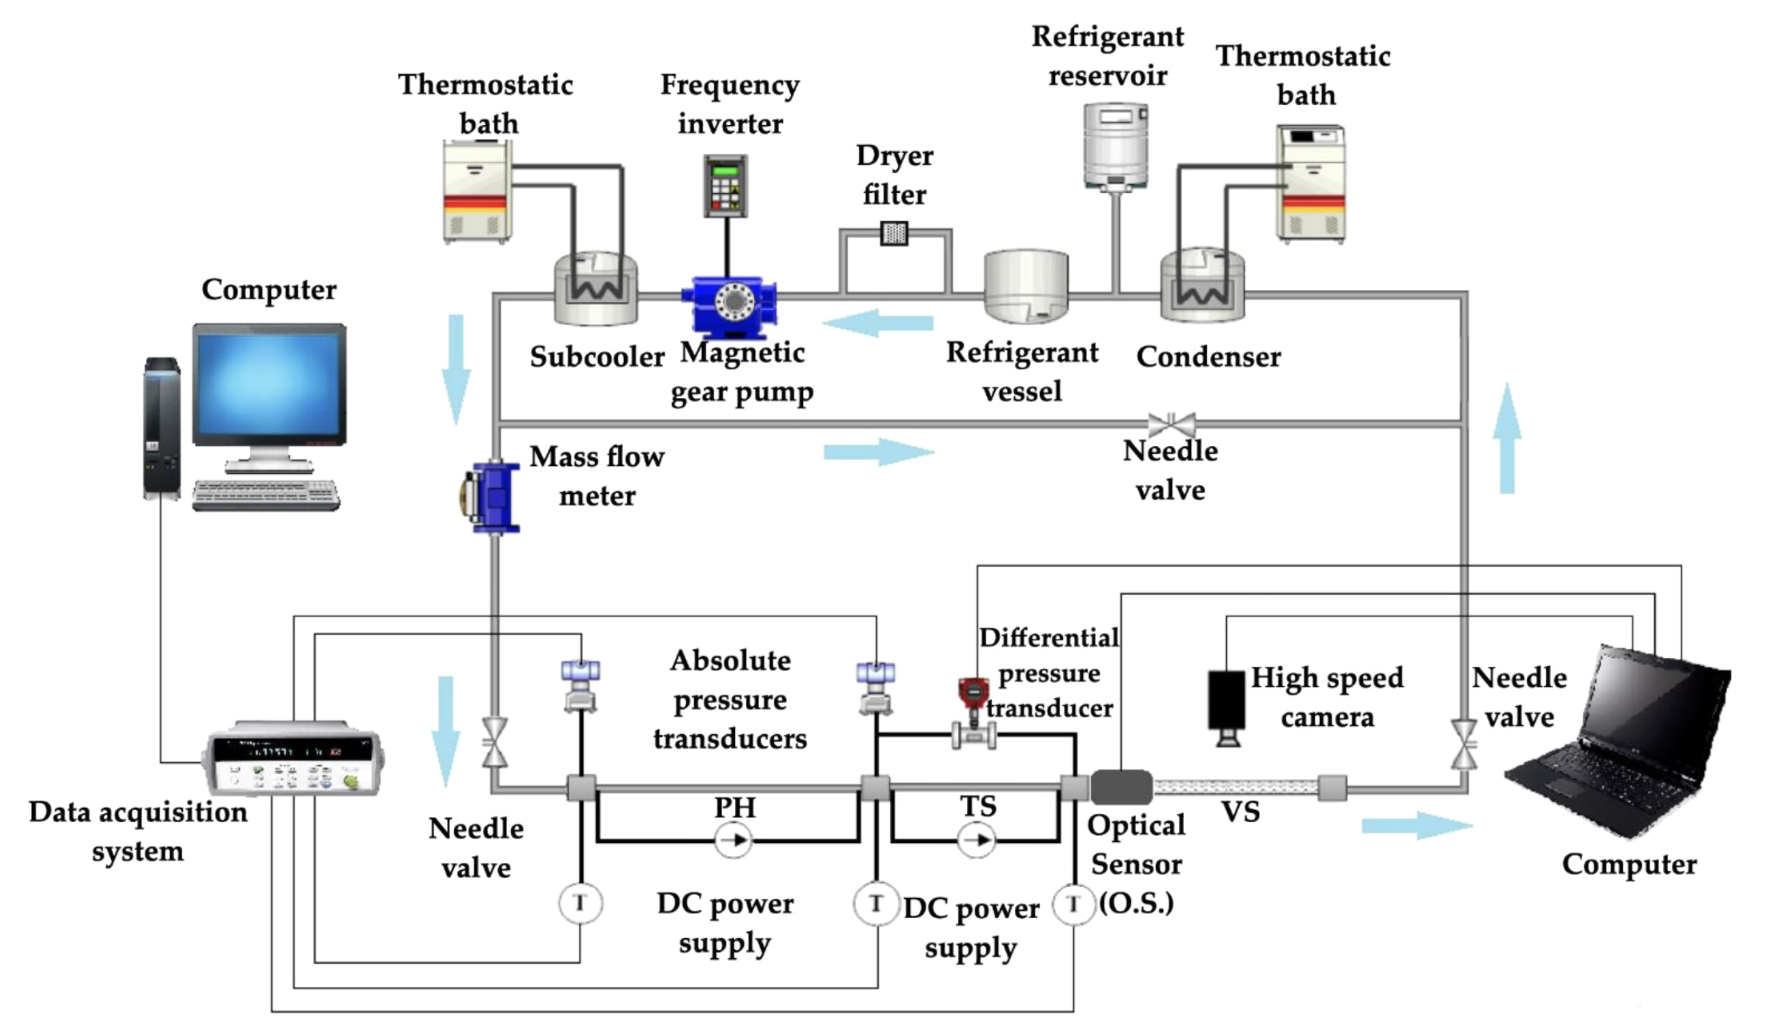
\includegraphics[width=\linewidth]{figuras/deoliveira2021-fig1-arranjo}
  \fonte{Adaptado de \citeonline{deoliveira2021}.}
  \end{minipage}
\end{figure}

\paragraph{Pré-aquecedor e seção de teste.}
O pré-aquecedor (PH) e a seção de teste (TS) são tubos horizontais de aço inoxidável com
diâmetro interno de 1,0\,mm, aquecidos por efeito Joule com aplicação direta de corrente
elétrica controlada por fonte de corrente contínua (SORENSEN\texttrademark{} DCS~8-125E).
O PH tem comprimento total de 515\,mm (440\,mm
aquecidos) e estabelece a condição termodinâmica na entrada da TS. A TS tem comprimento
total de 366\,mm (265\,mm aquecidos). O aquecimento permite estabelecer diferentes
condições de ebulição na saída da TS. A jusante da TS há uma seção de
visualização (VS) de tubo de vidro com 136\,mm e mesmo diâmetro interno, onde os padrões
são registrados visualmente e o sensor óptico é posicionado \cite{deoliveira2019,deoliveira2021}.

\paragraph{Sensor óptico (OS).}
Para a análise temporal dos padrões de escoamento, foi construído um sensor óptico (OS)
que detecta a refração e a variação de luminosidade da luz na interface
líquido-vapor \cite{deoliveira2019}.
Um LED de alta luminosidade ilumina o tubo transversalmente. Um resistor dependente de luz
(LDR) no lado oposto detecta a variação de transmitância óptica causada pela passagem das
fases. A variação de resistência do LDR é convertida em tensão por um circuito com filtro
passa-baixas de quarta ordem e amplificador operacional OPA\,4227, e o sinal é adquirido
pelo módulo NI\,6009 via LabVIEW\,2013. O sensor é posicionado no início da VS, registrando
as condições da saída da TS. Por responder ao que passa pelo feixe do LED em um dado instante,
o OS captura eventos locais associados à morfologia da interface: a passagem de
bolhas e frentes de vapor modifica o sinal. No padrão \textit{dispersed bubbles}, os autores
associaram a resposta do OS à sobreposição dos sinais produzidos pela passagem de várias bolhas
\cite{deoliveira2021}.

\paragraph{Transdutor de pressão diferencial (PD).}
A queda de pressão na TS é medida pelo transdutor ABB\texttrademark{} 600T, com frequência
de resposta de 10\,kHz \cite{deoliveira2021}. O PD mede a diferença de pressão ao
longo da seção de teste, enquanto o OS observa a transmissão óptica na seção de
visualização. Nos ensaios relatados, as frequências características do PD foram
geralmente menores que as do OS \cite{deoliveira2021}. Essa diferença observada
não equivale a uma limitação da frequência nominal de resposta do transdutor.

\paragraph{Aquisição e parâmetros experimentais.}
Nos ensaios de \citeonline{deoliveira2021}, os sinais do OS e do PD foram adquiridos
\textit{simultaneamente} a 1\,kHz, com 8.000 amostras por ensaio (8\,s por condição de operação).
Os padrões também foram registrados na seção de visualização por uma câmera de alta velocidade.
Os parâmetros dos
ensaios de referência estão resumidos no \autoref{qua:params-exp}.

\begin{quadro}[!htbp]
  \centering
  \begin{threeparttable}
  \caption{Parâmetros experimentais dos ensaios de \citeonline{deoliveira2021}.}
  \label{qua:params-exp}
  \begin{tabular}{ll}
    \hline
    \textbf{Parâmetro}                                        & \textbf{Valor(es)}           \\
    \hline
    Fluido de trabalho                                        & R600a (isobutano)            \\
    Temperatura de saturação [\textdegree{}C]                 & 27                           \\
    Fluxo mássico $G$ [kg/(m\textsuperscript{2}s)]           & 380, 510, 640, 760 e 890     \\
    Fluxo de calor na TS $q''$ [kW/m\textsuperscript{2}]     & 1, 5, 10, 20, 40 e 80        \\
    Frequência de aquisição [kHz]                             & 1                            \\
    Amostras por ensaio                                       & 8.000 (8\,s)                 \\
    Frequência de resposta do transdutor PD [kHz]            & 10                           \\
    \hline
  \end{tabular}
  \fonte{\citeonline{deoliveira2021}.}
  \end{threeparttable}
\end{quadro}

As sequências de quadros da câmera de alta velocidade registradas para cada condição de
fluxo mássico $G$ e fluxo de calor $q''$ constituíram os dados utilizados neste trabalho: delas se
reconstruiu o sinal espacial de brilho sobre o qual se calculou a coerência \textit{Wavelet}
alternativa, conforme detalhado no \autoref{cap:metodologia}.

\subsubsection{Padrões de escoamento e suas características}\label{sec:padroes}

Os padrões de escoamento observados no microtubo de 1\,mm com isobutano R600a são
descritos a seguir com base em \citeonline{deoliveira2021} e \citeonline{dias2025knn},
desde \textit{dispersed bubbles} até \textit{wavy annular} e \textit{smooth annular}. As faixas
espectrais apresentadas referem-se aos sinais de PD e OS do primeiro estudo e às
condições nele investigadas.
Neste trabalho, utilizaram-se os padrões da classificação manual dos ensaios.
A \autoref{fig:padroes-escoamento} ilustra cinco desses padrões.

\begin{figure}[!htbp]
  \centering
  \begin{minipage}{0.90\textwidth}
  \caption[Padrões de escoamento observados no LETEF.]{Padrões de escoamento
  observados no LETEF: (a) \textit{dispersed bubbles}, (b) \textit{plug}, (c) \textit{slug},
  (d) \textit{churn} e (e) \textit{wavy annular}.}
  \label{fig:padroes-escoamento}
  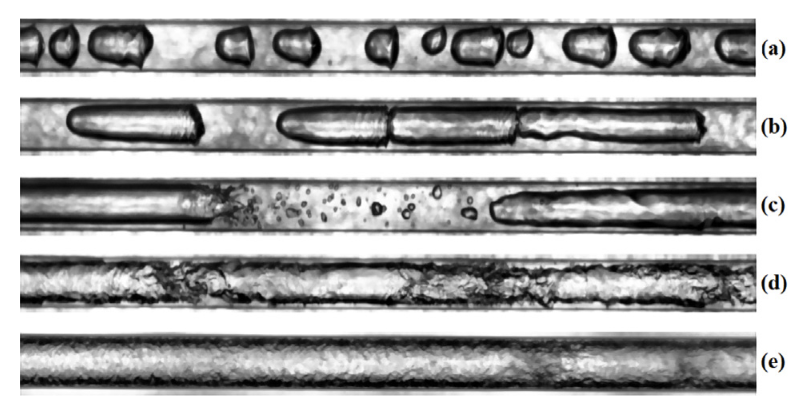
\includegraphics[width=\linewidth]{figuras/dias2025knn-fig4-padroes}
  \fonte{Adaptado de \citeonline{dias2025knn}.}
  \end{minipage}
\end{figure}

\textbf{\textit{Dispersed bubbles}}: esse padrão foi observado com baixo título de vapor $x$,
apenas para o fluxo mássico $G=890\,\text{kg/(m}^2\text{s)}$ e o fluxo de calor
$q''=1\,\text{kW/m}^2$ nos ensaios de \citeonline{deoliveira2021}. Pequenas bolhas ficam
dispersas na fase líquida, com diâmetro menor que o tubo. Nessa condição, o sinal de pressão
diferencial apresentou múltiplos picos entre 6 e 100\,Hz, e o sensor óptico apresentou
energia entre 4 e 35\,Hz. A análise por \textit{Wavelet} mostrou que as frequências
predominantes apareceram de forma intermitente nos dois sinais \cite{deoliveira2021}.

\textbf{\textit{Plug}}: foi observado principalmente em baixos
fluxos de calor $q''$ \cite{deoliveira2021}. As bolhas crescem e assumem forma cilíndrica, com
diâmetro próximo ao do tubo e comprimento maior que o diâmetro, motivo pelo qual esse padrão
também é chamado de \textit{elongated bubble flow} \cite{deoliveira2021}.
Nos ensaios relatados, também ocorreram bolhas dispersas de forma intermitente
entre os \textit{plugs}. As frequências predominantes ficaram entre 0{,}5 e 1\,Hz no PD
e entre 2 e 16\,Hz no OS \cite{deoliveira2021}.

\textbf{\textit{Slug}}: formado pelo coalescimento de \textit{plugs} com o aumento do título de
vapor $x$ e da fração de vazio $\alpha$ nas condições investigadas
\cite{deoliveira2021}. Alterna seções de
líquido e bolsões alongados de vapor com diâmetro próximo ao do tubo
\cite{dias2025knn,deoliveira2021}. A interface é instável e libera
pequenas bolhas dispersas no líquido entre os bolsões. O estudo relatou predominância
de baixas frequências no PD. Para o fluxo mássico $G=510\,\text{kg/(m}^2\text{s)}$, os autores
relataram no OS um pico em 2{,}8\,Hz associado à passagem dos \textit{slugs}. Os autores
sugeriram que as componentes próximas de 8, 12, 23 e 32\,Hz poderiam resultar da passagem
de bolhas dispersas entre os \textit{slugs}. Essas frequências variaram com o fluxo mássico $G$.
A natureza caótica foi indicada pelos maiores expoentes de Lyapunov, positivos, entre 0{,}261
e 0{,}463 no PD e entre 0{,}413 e 4{,}362 no OS \cite{deoliveira2021}.

\textbf{\textit{Churn}}: regime de transição entre \textit{slug} e \textit{annular}
\cite{dias2025knn}.
Nos ensaios de \citeonline{deoliveira2021}, a maior velocidade do vapor foi associada à presença de
jatos e a instabilidades na interface. O sinal de pressão diferencial apresenta
frequências predominantes de baixa energia em 8\,Hz ou menos. No sensor óptico,
observaram-se componentes de baixa frequência e componentes mais altas, entre
15 e 28\,Hz, associadas pelos autores ao aumento do fluxo mássico $G$.


\textbf{\textit{Wavy annular}}: o vapor ocupa o centro
do tubo e o líquido forma um filme na parede
\cite{dias2025knn,deoliveira2021}, sobre o qual deslizam ondas frontais na interface
líquido-vapor \cite{deoliveira2021}. No exemplo analisado pelos autores, a CWT não
identificou frequências características no PD, enquanto o OS apresentou maior energia
entre 2 e 16\,Hz ao longo do tempo.
As flutuações de pressão apresentaram expoente de Hurst abaixo de 0{,}5, indicando
comportamento anti-persistente \cite{deoliveira2021}.

\textbf{\textit{Smooth annular}}: foi observado apenas na combinação
do menor fluxo mássico $G$ com o maior fluxo de calor $q''$ testados
\cite{deoliveira2021}. A interface entre o filme líquido e o núcleo de vapor é
praticamente sem ondas \cite{cheng2023}.
\citeonline{dias2025knn} limitaram a classificação a cinco padrões
de escoamento, não incluindo o \textit{smooth annular}.

As diferenças entre as respostas espectrais do PD e do OS
\cite{deoliveira2021} motivam investigar representações \textit{Wavelet}.
A utilidade da coerência alternativa para os panoramas foi avaliada neste trabalho.



% =========================================================
\subsection{Fração de vazio e representação das fases}\label{sec:fracao-vazio}
% =========================================================

Enquanto o título de vapor $x$ caracteriza a participação do vapor na vazão
mássica, a fração de vazio $\alpha$ expressa a parcela do volume da mistura ocupada
pela fase gasosa. Em escoamento líquido-vapor, essa definição pode ser escrita
como \cite{masiukiewicz2021}:

\begin{equation}\label{eq:fracao-vazio-volume}
  \alpha=\frac{V_v}{V_v+V_l}.
\end{equation}

\noindent
O volume de vapor $V_v$ e o volume de líquido $V_l$ se referem à mesma região
de observação. A fração de vazio $\alpha$ é adimensional: o valor zero
representa somente líquido, e o valor um, somente vapor.

Em uma mesma seção do tubo, a relação entre o título de vapor $x$ e a
fração de vazio $\alpha$ depende das massas específicas e das velocidades médias de cada fase
\cite{deoliveira2021}. A mesma ocupação em volume pode, portanto,
corresponder a participações diferentes na vazão mássica. Por isso, a
proporção de gás identificada nas imagens não determina, por si só,
o título de vapor $x$.

Na análise de imagens, uma máscara binária atribui cada pixel a uma das
fases. A contagem desses pixels fornece uma proporção de área na projeção
observada, como no procedimento de \citeonline{schepperle2024}.
Uma projeção lateral, porém, não informa diretamente a extensão da fase
na profundidade do tubo. A conversão das larguras observadas em áreas de
seções circulares exige uma hipótese geométrica adicional, explicitada na
metodologia. Assim, a estimativa obtida por esse procedimento permanece
condicionada à geometria assumida e à identificação das interfaces.
Os valores de fração de vazio relatados na literatura não foram empregados
como calibração das estimativas obtidas nesse trabalho.

A fração média, isoladamente, não determina a forma ou a distribuição das
estruturas de gás. \citeonline{masiukiewicz2021} destacaram essa limitação ao
combinar a fração volumétrica com parâmetros de tamanho, distribuição e
superfície interfacial. Na análise por \textit{Wavelet},
\citeonline{nguyen2010} também utilizaram a fração de vazio média junto ao
coeficiente de energia \textit{Wavelet} local efetiva na identificação de bolhas discretas
e de casos de \textit{churn}. Esses antecedentes motivam examinar
descritores complementares: a estimativa de fração de vazio resume a
ocupação de vapor, as transições da máscara descrevem as alternâncias
espaciais detectadas e os perfis \textit{Wavelet} caracterizam a distribuição
das variações de intensidade por escala. Essa relação conceitual não
transforma o sinal de intensidade em uma medição calibrada de fração de vazio.

% ---------------------------------------------------------
\subsection{Transformada \textit{Wavelet}}\label{sec:wavelet}
% ---------------------------------------------------------

A transformada \textit{Wavelet} permite examinar como o conteúdo de um sinal
varia ao longo do tempo. Enquanto o espectro de Fourier global resume as
frequências presentes no registro completo, a análise \textit{Wavelet} localiza essas
componentes no sinal. Para isso, utiliza versões dilatadas e deslocadas de uma
função oscilatória localizada, a \textit{Wavelet} mãe. Escalas pequenas favorecem a
localização de variações rápidas. Escalas grandes permitem distinguir melhor
componentes de baixa frequência \cite{torrence1998}. Essa propriedade permite
examinar variações locais nos sinais de escoamento bifásico.
O \autoref{qua:wavelet-fourier} compara as duas transformadas.

\begin{quadro}[!htbp]
  \centering
  \begin{threeparttable}
  \caption{Comparação entre a transformada de Fourier e a transformada \textit{Wavelet}.}
  \label{qua:wavelet-fourier}
  \begin{tabular}{lll}
    \hline
    \textbf{Característica}       & \textbf{Fourier global} & \textbf{\textit{Wavelet} contínua}   \\
    \hline
    Localização temporal          & Não                  & Sim                            \\
    Informação principal          & Espectro global      & Conteúdo por tempo e escala    \\
    Janela de análise              & Registro completo    & Duração variável com a escala  \\
    Variação ao longo do tempo     & Não localizada       & Representada no mapa           \\
    \hline
  \end{tabular}
  \fonte{Adaptado de \citeonline{torrence1998}.}
  \end{threeparttable}
\end{quadro}

\subsubsection{Transformada \textit{Wavelet} Contínua (CWT)}\label{sec:cwt}

A CWT de um sinal $x(t)$ em relação à \textit{Wavelet}-mãe $\psi$ é definida
na forma integral por \cite{schuck2019}:

\begin{equation}\label{eq:cwt}
  W(a, b) = \frac{1}{\sqrt{a}} \int_{-\infty}^{\infty} x(t)\,
  \psi^*\!\left(\frac{t - b}{a}\right) dt,
\end{equation}

\noindent
O coeficiente \textit{Wavelet} $W(a,b)$ quantifica a resposta do sinal à \textit{Wavelet} na escala $a$
e na posição $b$. A escala $a>0$ controla a duração da função de análise,
enquanto a posição $b$ determina onde ela é centrada no sinal. A integral reúne os
produtos entre o sinal e a conjugada complexa dessa função. O fator
$1/\sqrt{a}$ preserva a energia da \textit{Wavelet} ao variar a escala.
Escalas grandes correspondem a baixas frequências, e escalas pequenas,
a altas frequências. A adaptação ao domínio espacial
e a conversão das escalas em comprimentos de onda são descritas na
\autoref{sec:met-wco-morlet}.

O escalograma permite visualizar como o conteúdo do sinal varia ao longo do
tempo e entre escalas \cite{torrence1998}. Exemplos dos padrões
\textit{slug} e \textit{churn} para os dois canais do arranjo experimental
(\autoref{fig:scalogram-slug} a \autoref{fig:scalogram-churn-os}) estão apresentados
na \autoref{sec:wps-wcs-wco}.

A \textit{Wavelet} de Morlet complexa combina oscilações com uma envoltória
gaussiana e pode ser escrita na forma aproximada
\cite{torrence1998,schuck2019}:

\begin{equation}\label{eq:morlet}
  \psi(t) = \pi^{-1/4}\, e^{-t^2/2}\, e^{j\omega_0 t},
\end{equation}

\noindent
em que a coordenada $t$ é adimensional, a unidade imaginária é $j=\sqrt{-1}$ e
o fator $\pi^{-1/4}$ normaliza a energia.
Neste trabalho, adotou-se a frequência angular central adimensional
$\omega_0=6$ nessa forma aproximada
\cite{schuck2019}. Por ser complexa, a Morlet fornece coeficientes com módulo
e fase, permitindo estudar a relação entre dois sinais \cite{torrence1998}.
A \autoref{fig:morlet-mae} apresenta suas partes real e imaginária, cujas
oscilações diminuem em amplitude ao se afastarem da origem.

\begingroup
\setlength{\intextsep}{12pt}
\begin{figure}[!ht]
  \centering
  \caption[\textit{Wavelet} mãe de Morlet complexa utilizada na análise.]{Partes real
  e imaginária da \textit{Wavelet} mãe de Morlet complexa (\autoref{eq:morlet}), com
  $\omega_0=6$, $a=1$ e $b=0$. Eixos adimensionais.}
  \label{fig:morlet-mae}
  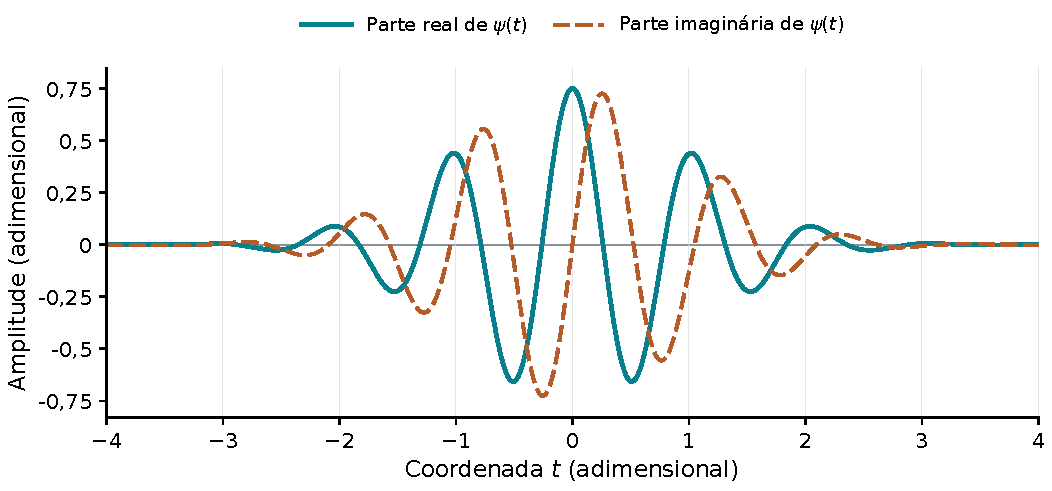
\includegraphics[width=\textwidth]{figuras/morlet_mae.pdf}
  \fonte{Elaborada pelo autor (2026).}
\end{figure}
\endgroup

\subsubsection{Espectro de Potência, Espectro Cruzado e Coerência \textit{Wavelet}}\label{sec:wps-wcs-wco}

A partir da CWT, o espectro de potência descreve as componentes de cada sinal,
o espectro cruzado reúne informações de dois sinais e a coerência quantifica
sua associação por uma medida normalizada \cite{torrence1998}.

\paragraph{Espectro de Potência \textit{Wavelet} (WPS).}
O WPS descreve a distribuição da potência do sinal $x$ entre posições e escalas:

\begin{equation}\label{eq:wps}
  P_x(a, b) = |W_x(a, b)|^2.
\end{equation}

Valores elevados da potência \textit{Wavelet} $P_x(a,b)$ localizam componentes com maior potência
na escala $a$ e na posição $b$.
A média temporal do WPS fornece o espectro \textit{Wavelet} global, comparável a
uma versão suavizada do espectro de Fourier \cite{torrence1998}.

\begingroup
\sloppy
Para ilustrar a interpretação do espectro de potência \textit{Wavelet} $P_x(a,b)$,
apresentam-se os escalogramas de \citeonline{deoliveira2021}, obtidos a partir dos sinais
de pressão diferencial (PD) e do sensor óptico (OS) nos padrões \textit{slug} e
\textit{churn}. Esses mapas mostram como a potência \textit{Wavelet} $P_x(a,b)$
se distribui entre frequências e varia ao longo do tempo.
\par
\endgroup

A \autoref{fig:scalogram-slug} e a \autoref{fig:scalogram-churn} mostram os escalogramas
do WPS do PD para \textit{slug} e \textit{churn}. A \autoref{fig:scalogram-slug-os}
e a \autoref{fig:scalogram-churn-os} apresentam os correspondentes do OS.
Esses exemplos permitem comparar dois padrões pelo mesmo sensor e as respostas
dos dois sensores a um mesmo padrão. Os mapas apresentam distribuições diferentes
de energia e componentes em faixas sobrepostas. O estudo relatou, em geral,
frequências características menores no PD do que no OS \cite{deoliveira2021}.

\begin{figure}[!htbp]
  \centering
  \begin{minipage}{0.85\textwidth}
  \caption[WPS da pressão diferencial no padrão \textit{slug}.]{WPS da pressão
  diferencial em \textit{slug}: (a) sinal e (b, c) escalogramas e perfis de potência
  média. Fluxo mássico $G$ ($\mathrm{kg\,m^{-2}\,s^{-1}}$): (a, c) 760 e (b) 510.}
  \label{fig:scalogram-slug}
  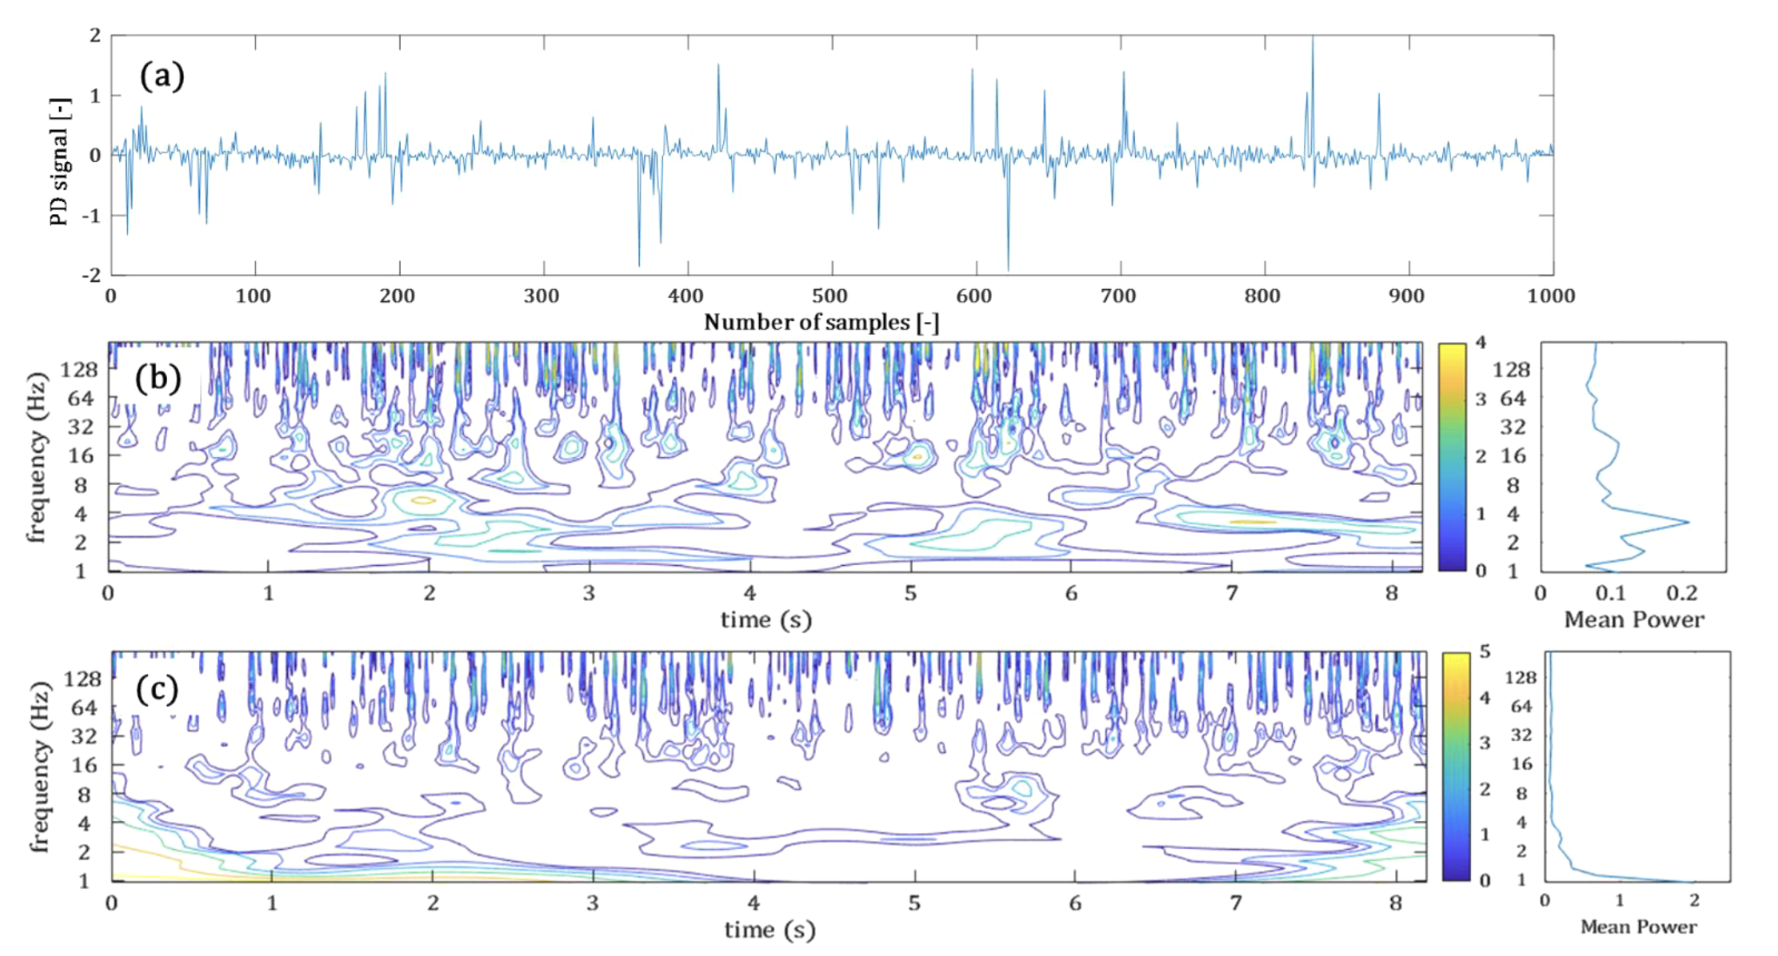
\includegraphics[width=\linewidth]{figuras/deoliveira2021-fig13-slug-pd}
  \fonte{Adaptado de \citeonline{deoliveira2021}.}
  \end{minipage}
\end{figure}

\begin{figure}[!htbp]
  \centering
  \begin{minipage}{0.85\textwidth}
  \caption[WPS do sensor óptico no padrão \textit{slug}.]{WPS do sensor óptico
  em \textit{slug}: (a) sinal e (b, c) escalogramas e perfis de potência média.
  Fluxo mássico $G$ ($\mathrm{kg\,m^{-2}\,s^{-1}}$): (a, c) 760 e (b) 510.}
  \label{fig:scalogram-slug-os}
  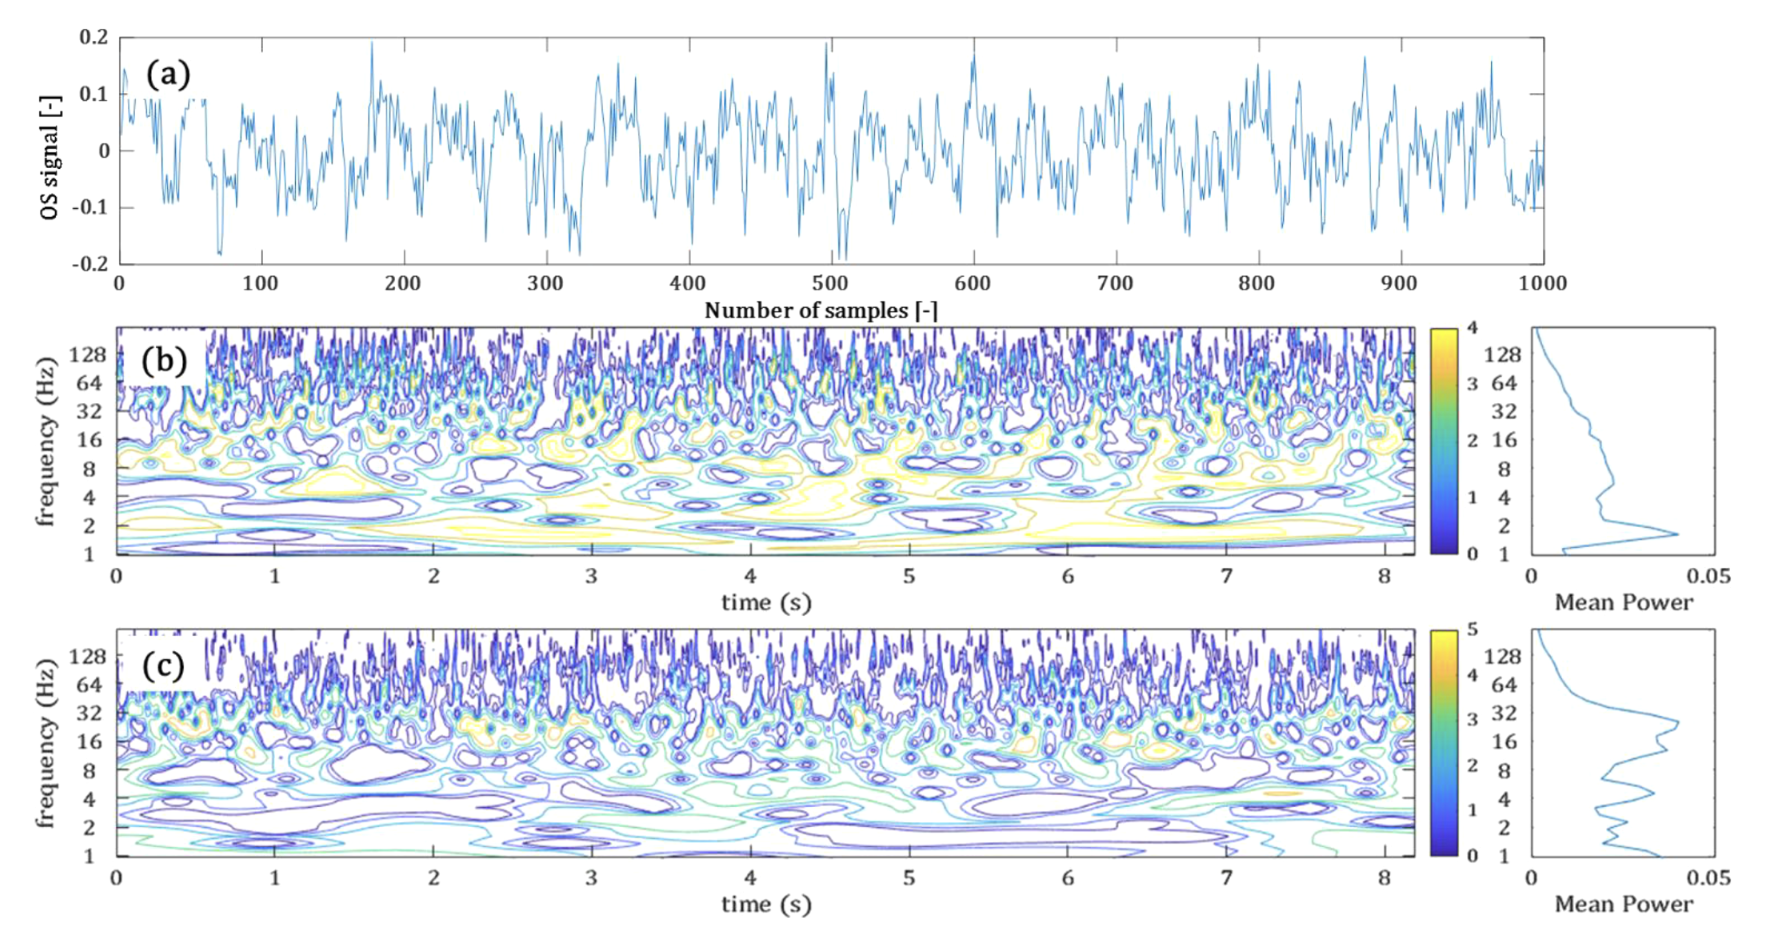
\includegraphics[width=\linewidth]{figuras/deoliveira2021-fig14-slug-os}
  \fonte{Adaptado de \citeonline{deoliveira2021}.}
  \end{minipage}
\end{figure}

\begin{figure}[!htbp]
  \centering
  \begin{minipage}{0.85\textwidth}
  \caption[WPS da pressão diferencial no padrão \textit{churn}.]{WPS da pressão
  diferencial em \textit{churn}: (a) sinal e (b, c) escalogramas e perfis de potência
  média. Fluxo mássico $G$ ($\mathrm{kg\,m^{-2}\,s^{-1}}$): (a, b) 510 e (c) 760.}
  \label{fig:scalogram-churn}
  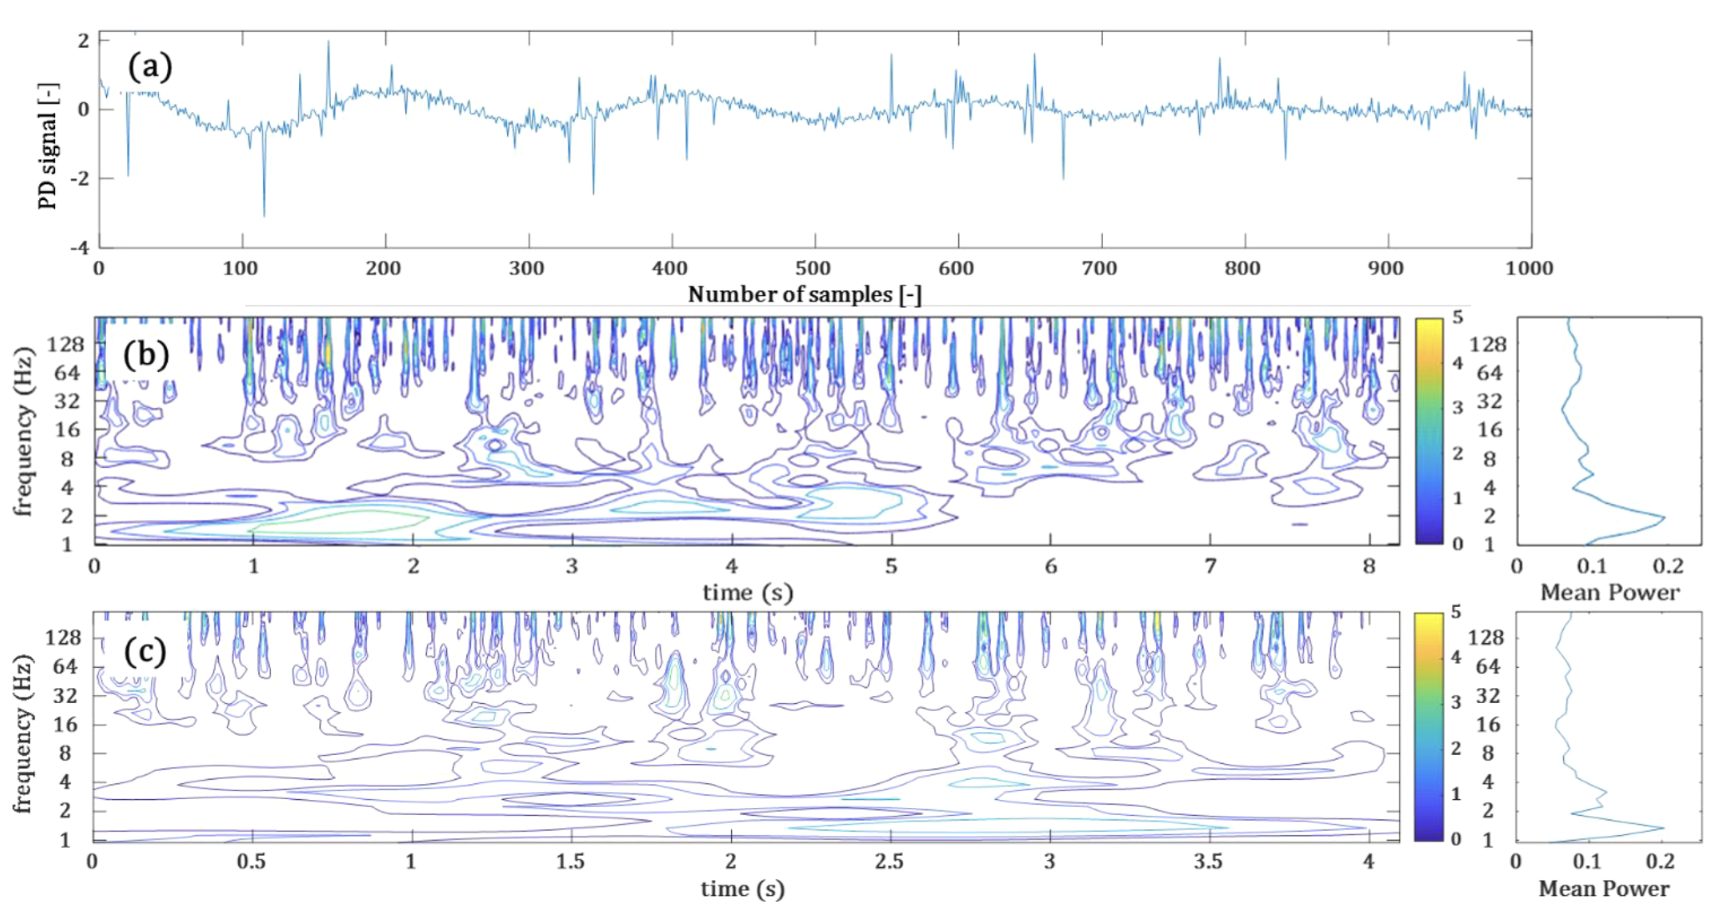
\includegraphics[width=\linewidth]{figuras/deoliveira2021-fig17-churn-pd}
  \fonte{Adaptado de \citeonline{deoliveira2021}.}
  \end{minipage}
\end{figure}

\begin{figure}[!htbp]
  \centering
  \begin{minipage}{0.85\textwidth}
  \caption[WPS do sensor óptico no padrão \textit{churn}.]{WPS do sensor óptico
  em \textit{churn}: (a) sinal e (b, c) escalogramas e perfis de potência média.
  Fluxo mássico $G$ ($\mathrm{kg\,m^{-2}\,s^{-1}}$): (b) 510 e (c) 760.}
  \label{fig:scalogram-churn-os}
  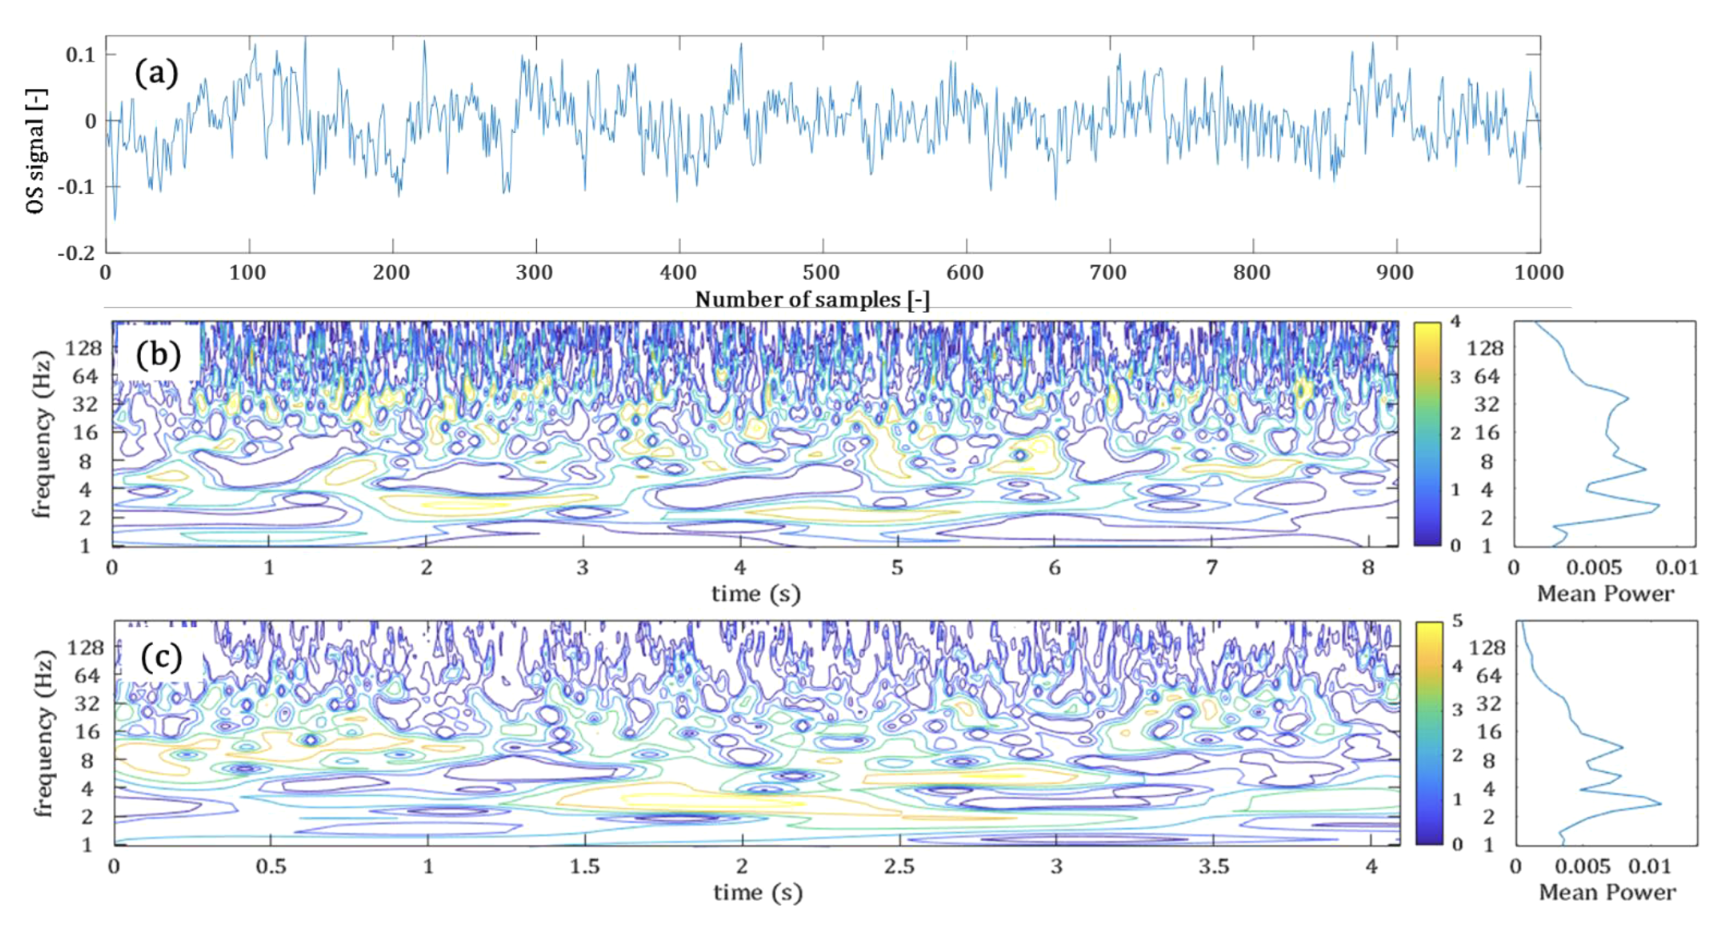
\includegraphics[width=\linewidth]{figuras/deoliveira2021-fig18-churn-os}
  \fonte{Adaptado de \citeonline{deoliveira2021}.}
  \end{minipage}
\end{figure}


\paragraph{Espectro Cruzado \textit{Wavelet} (WCS).}
O WCS mede a relação entre dois sinais $x$ e $y$ no domínio tempo-escala:

\begin{equation}\label{eq:wcs}
  C_{xy}(a, b) = W_x(a, b) \cdot W_y^*(a, b).
\end{equation}

O produto combina os coeficientes dos dois sinais na mesma escala e posição.
Seu módulo destaca regiões de potência comum, e sua fase descreve a defasagem
relativa entre as componentes \cite{torrence1998,grinsted2004}.
Como o WCS ainda depende das amplitudes dos sinais, potência comum elevada
não equivale, por si só, a coerência elevada. A conversão da diferença de
fase em atraso temporal depende da frequência analisada \cite{grinsted2004}.

\paragraph{Coerência \textit{Wavelet} (WCO).}
A coerência \textit{Wavelet} clássica $\gamma_{xy}$ é uma medida quadrática de associação,
com valores entre 0 e 1 quando o denominador é positivo:

\begin{equation}\label{eq:wco-classica}
  \gamma_{xy}(a, b) = \frac{|S\bigl[a^{-1}C_{xy}(a, b)\bigr]|^2}
                           {S\bigl[a^{-1}P_x(a, b)\bigr] \cdot S\bigl[a^{-1}P_y(a, b)\bigr]},
\end{equation}

\noindent
A normalização compara o espectro cruzado \textit{Wavelet} $C_{xy}(a,b)$ com os
espectros de potência \textit{Wavelet} $P_x(a,b)$ e $P_y(a,b)$, considerando a potência
presente em cada sinal. A suavização $S[\cdot]$ calcula médias ponderadas em uma
pequena região do mapa, reunindo instantes próximos e escalas semelhantes.
Antes dessas médias, aplica-se o fator de ponderação $a^{-1}$, correspondente ao
inverso da escala $a$. Assim, a coerência \textit{Wavelet} clássica $\gamma_{xy}(a,b)$
descreve a associação entre as oscilações dos dois sinais nessa região.
Valores da coerência \textit{Wavelet} clássica $\gamma_{xy}(a,b)$ próximos de 1 indicam
forte associação linear local, enquanto valores da coerência \textit{Wavelet}
clássica $\gamma_{xy}(a,b)$ próximos de zero indicam associação linear local fraca
\cite{grinsted2004}.

\paragraph{Formulação alternativa de Schuck e Bodmann.}

Sem a suavização $S[\cdot]$, a coerência \textit{Wavelet} clássica $\gamma_{xy}(a,b)$
seria calculada isoladamente em cada ponto do mapa. Nesse caso, a identidade
$|W_xW_y^*|^2=|W_x|^2|W_y|^2$ faria o numerador e o denominador da
\autoref{eq:wco-classica} terem o mesmo valor. A divisão resultaria, portanto, em 1
sempre que o denominador fosse diferente de zero, mesmo para sinais sem relação
física entre si. Esse resultado decorreria da própria fórmula e não demonstraria
uma associação entre os sinais \cite{torrence1998}. Ao reunir valores vizinhos antes
da divisão, a suavização $S[\cdot]$ evita esse resultado automaticamente igual a 1.
A coerência \textit{Wavelet} clássica $\gamma_{xy}(a,b)$ passa, então, a representar a
associação em uma pequena região de tempo e escala ao redor de cada ponto
\cite{grinsted2004}.

\citeonline{schuck2019} formularam uma alternativa baseada na CWT das funções de
correlação. Para processos estacionários, definiram a autocorrelação e a correlação
cruzada pela esperança matemática:

\begin{equation}\label{eq:autocorr}
  R_{xx}(\tau)=\operatorname{E}\{x(t+\tau)x^*(t)\},
\end{equation}

\begin{equation}\label{eq:crosscorr}
  R_{xy}(\tau)=\operatorname{E}\{x(t+\tau)y^*(t)\}.
\end{equation}

\noindent
A autocorrelação $R_{xx}(\tau)$ compara um sinal com uma versão deslocada
de si mesmo, enquanto a correlação cruzada $R_{xy}(\tau)$ compara dois sinais
separados pelo atraso $\tau$. A esperança matemática $\operatorname{E}\{\cdot\}$
representa a média estatística teórica desses produtos, com o conjugado complexo
do segundo fator. Sob a hipótese de estacionariedade, essas funções
dependem do atraso, sem depender da origem temporal $t$ \cite{schuck2019}.

Neste trabalho, as autocorrelações estimadas $\widehat R_{xx}$ e
$\widehat R_{yy}$ e a correlação cruzada estimada $\widehat R_{xy}$ foram
calculadas com um registro de cada sinal por comparação. O chapéu indica
que esses valores foram estimados a partir dos dados. Aplicou-se então a CWT
a essas funções, seguindo a formulação de \citeonline{schuck2019}:

\begin{equation}\label{eq:wps-alt}
  \widetilde P_x(a,b)=\left|W_{\widehat R_{xx}}(a,b)\right|,
  \qquad
  \widetilde P_y(a,b)=\left|W_{\widehat R_{yy}}(a,b)\right|,
\end{equation}

\begin{equation}\label{eq:wcs-alt}
  \widetilde C_{xy}(a,b)=W_{\widehat R_{xy}}(a,b),
\end{equation}

\begin{equation}\label{eq:wco-alt}
  \widetilde\gamma_{xy}(a,b)=
  \frac{|\widetilde C_{xy}(a,b)|^2}
       {\widetilde P_x(a,0)\,\widetilde P_y(a,0)}.
\end{equation}

\noindent
O coeficiente \textit{Wavelet} $W_{\widehat R_{xx}}(a,b)$ resulta da CWT da
autocorrelação estimada $\widehat R_{xx}$. Seu módulo fornece a potência
alternativa $\widetilde P_x(a,b)$, com cálculo análogo para a potência
alternativa $\widetilde P_y(a,b)$. A escala $a$ controla a dilatação da
\textit{Wavelet}, enquanto a posição $b$ indica onde ela é centrada no eixo
do atraso da correlação $\tau$. A CWT da correlação cruzada estimada $\widehat R_{xy}$
fornece o espectro cruzado complexo $\widetilde C_{xy}(a,b)$, que conserva
módulo e fase \cite{schuck2019}.

Na \autoref{eq:wco-alt}, divide-se o módulo ao quadrado do espectro cruzado
alternativo $\widetilde C_{xy}(a,b)$ pelo produto das potências alternativas
$\widetilde P_x(a,0)$ e $\widetilde P_y(a,0)$. Esses valores correspondem à
mesma escala $a$ e ao atraso nulo $b=0$, onde ocorrem os máximos com a Morlet
adotada. A coerência alternativa $\widetilde\gamma_{xy}(a,b)$ só é definida
quando esse produto é positivo. O mapa descreve a associação por escala $a$
e atraso relativo $b$, sem localizar o instante original de ocorrência de
um evento \cite{schuck2019}. Na aplicação deste trabalho, o atraso $b$ foi
expresso em pixels do panorama reconstruído.

A formulação pressupõe processos estacionários e depende das correlações
estimadas a partir dos registros disponíveis. A aplicação da CWT a essas
correlações dispensa a suavização da definição clássica, mas mantém a
incerteza associada à estimação \cite{schuck2019}. O procedimento discreto
adotado neste trabalho é apresentado na \autoref{sec:met-wco}.

O \autoref{qua:wco-comparativo} resume as diferenças relevantes para a leitura
dos mapas.

\begin{quadro}[!htbp]
  \centering
  \begin{threeparttable}
  \caption[Comparação entre as formulações clássica e alternativa da coerência
  \textit{Wavelet}.]{Formulações clássica e alternativa da coerência
  \textit{Wavelet}, conforme \citeonline{torrence1998},
  \citeonline{grinsted2004} e \citeonline{schuck2019}.}
  \label{qua:wco-comparativo}
  \begin{tabular}{p{3.1cm}p{5.1cm}p{5.1cm}}
    \hline
    \textbf{Aspecto} & \textbf{Clássica} & \textbf{Alternativa} \\
    \hline
    Entrada da CWT & Sinais diretamente & Funções de correlação estimadas \\
    Potência & $|W_x(a,b)|^2$ & $|W_{\widehat R_{xx}}(a,b)|$ \\
    Espectro cruzado & $W_x(a,b)W_y^*(a,b)$ & $W_{\widehat R_{xy}}(a,b)$ \\
    Normalização & Espectros suavizados em tempo e escala & Potências no atraso nulo da mesma escala \\
    Coordenada $b$ & Posição no sinal & Atraso da correlação \\
    Interpretação & Associação localizada no tempo & Associação por escala e atraso \\
    \hline
  \end{tabular}
  \fonte{Elaborada pelo autor (2026).}
  \end{threeparttable}
\end{quadro}

\citeonline{schuck2019} avaliaram a formulação com sinais sintéticos contendo
pulsos gaussianos modulados e ruído gaussiano, com razão sinal-ruído de 5\,dB e
atraso conhecido de 500 amostras entre os pulsos. Nos exemplos apresentados,
a formulação alternativa permitiu identificar o atraso e a escala dos
transientes mesmo na presença de eventos adicionais não correlacionados.

Neste trabalho, a formulação foi aplicada aos sinais de intensidade extraídos
dos panoramas. Essa aplicação exigiu considerar as condições de reconstrução
das imagens, pois as emendas entre as tiras de quadros podem introduzir
variações no sinal analisado. O \autoref{cap:metodologia} apresenta o
procedimento de reconstrução dos panoramas e as etapas de análise desses sinais.
